\documentclass[12pt]{article}
\usepackage[total={6in, 10in}]{geometry}

%langue
\usepackage[T1, T2A]{fontenc}
\usepackage[utf8]{inputenc}
\usepackage[english, ukrainian]{babel}

%math symbol
\usepackage{amssymb}
\usepackage{amsmath}
\usepackage{textcomp}
\usepackage{gensymb} %for degree

%image include
\usepackage{graphicx}

\author{ФФ-93 Недождій Олексій}

\date{}

\title{Лабораторна робота №4\\
p--n перехід}


\begin{document}
\maketitle

\section{Теоретичні відомості}

\subsection{Вольт Амперної характеристика діода}
Вольт-амперна  характеристика діода досить описується формулою:
\[
    I = I_s \left( e^{\dfrac{U}{m \varphi_{{\scriptscriptstyle T}}}} - 1 \right),
\]

де $I_s$ -- струм насичення, визначається типом напівпровідника

$\varphi_{\scriptscriptstyle T} = \dfrac{k T}{e_0}$ -- термічний(температурний) потенціал (при $t = 12^{\circ}C$\\
$\hspace*{10cm}\varphi_T \approx 24.6\text{млВ})$

$m$ -- поправочний коефіцієнт,  що  характеризує  плавність  і  товщину  p--n  -
переходу.

\[
    m = U \frac{1}{\varphi_t ln(\frac{I}{I_s} + 1)}
\]

Статистична похибка вимірювання розраховувалась за формулою :
\[
    \delta{\text{ст}_m} = \frac{1}{4}\sqrt{\sum_{i=1}^{4}(m_i - \overline{m})^2}
\]
Систематична похибка вимірювання розраховувалась за формулою :
\[
    \delta_{\text{сис}_m} =
    \sqrt{ (\frac{\partial m}{\partial U} \delta_{U})^2
    + (\frac{\partial m}{\partial \varphi_t} \delta_{\varphi_t})^2
    + (\frac{\partial m}{\partial I_s} \delta_{I_s})^2 } \; \text{, де}
\]

Тоді загальна похибка :
\[
    \Delta_m = \sqrt{\sigma_{\text{сис}}^2 + \sigma_{\text{ст}}^2}
\]

\subsection{Вольт-Фарадна характеристика діода}
Вольт-фарадна залежність описується за таким законом:
\[
    C(U) = C_0 {\left( \dfrac{\varphi_k}{\varphi_k + U} \right)}^{\nu}
\]

$C_0$ -- ємність діода при нульовій зворотній напрузі

$\varphi_k$ -- контактна різниця потенціалів

$\nu$ -- коефіцієнт, що залежить від типу варикапу.


\section{Вольт Амперної характеристика діода}

\newpage
\subsection{Перший діод}
\begin{table}[ht]
    \centering
	\caption{ВАХ першого діода}
    \begin{tabular}{lllllll}
        \hline
        $U$, В & $I_1$, мкА & $I_2$, мкА & $I_3$, мкА & $I_4$, мкА  & $\sigma_{\overline{I}}$ & $\Delta U$\\
        \hline
        0.00  & 5   & 5    & 5    & 5 & 0       & 0.005\\
        0.13  & 4   & 4    & 4    & 5 & 0.2     & 0.005\\
        0.15  & 5   & 5    & 5    & 5 & 0       & 0.005\\
        0.30  & 6   & 7    & 7    & 7 & 0.2     & 0.005\\
        0.35  & 12  & 14   & 14   & 15 & 0.5    & 0.005\\
        0.40  & 46  & 69   & 55   & 60 & 4.1    & 0.005\\
        0.42  & 101 & 100  & 120  & 113 & 4.1   & 0.005\\
        0.44  & 184 & 198  & 216  & 222 & 7.5   & 0.005\\
        0.46  & 359 & 390  & 410  & 445 & 15.6  & 0.005\\
        0.47  & 666 & 670  & 700  & 566 & 25.2  & 0.005\\
        0.48  & 890 & 894  & 920  & 890 & 6.2   & 0.005\\
        0.49  & 996 & 1000 & 1120 & 1140 & 33.2 & 0.005\\
        \hline
    \end{tabular}
\end{table}

\begin{figure}[!ht]
    \centering
    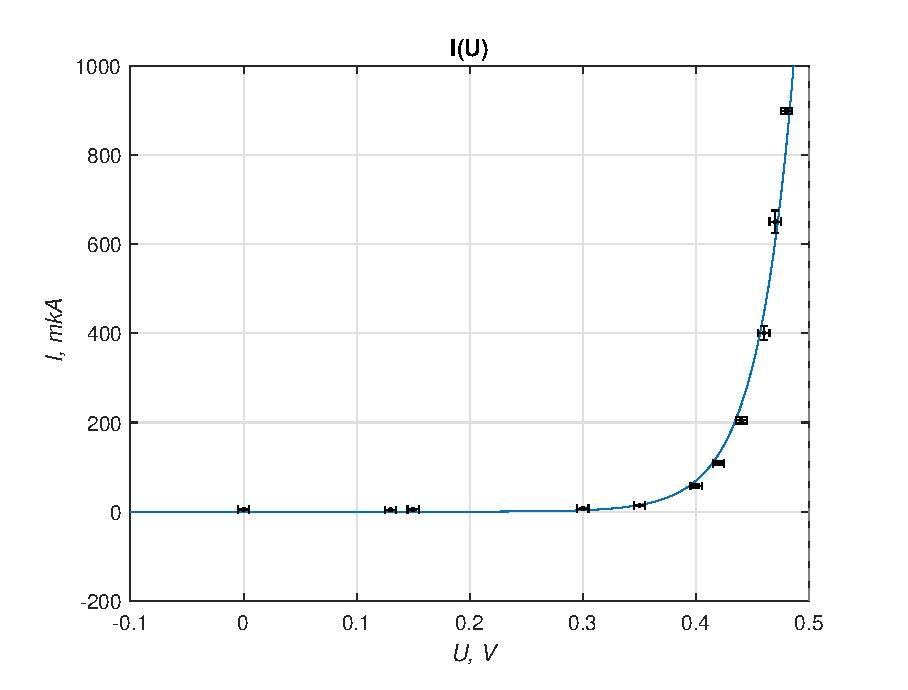
\includegraphics[scale=0.7]{vac0.eps}
\end{figure}


$\Delta I_s = \sqrt{0.007^2 + 0.002^2 + 0.005^{2}} = 0.009$нА

$\Delta m = \sqrt{0.02^{2} + 0.02^{2}} = 0.03$

$I_s = 0.323\; \text{нА} \pm 0.009 \text{нА}, \; m = 1.31 \pm 0.03$.


\newpage
\subsection{Другій діод}
\begin{table}[ht]
	\centering
	\caption{ВАХ другого діода}
	\begin{tabular}{llllllll}
		\hline
        $U$, В & $I_1$, мкА & $I_2$, мкА & $I_3$, мкА & $I_4$, мкА & $\sigma_{\overline{I}}$ &  $\Delta U$\\
		\hline
		0    & 4   & 5   & 4     & 5   & 0.2  & 0.005\\
        0.2  & 5   & 5   & 5     & 5   & 0    & 0.005\\
        0.3  & 7   & 7   & 7     & 8   & 0.2  & 0.005\\
        0.4  & 30  & 33  & 33    & 34  & 0.7  & 0.005\\
        0.42 & 50  & 50  & 50    & 53  & 0.6  & 0.005\\
        0.45 & 106 & 98  & 98    & 99  & 1.7  & 0.005\\
        0.47 & 146 & 146 & 150   & 152 & 1.3  & 0.005\\
        0.50 & 293 & 283 & 282   & 299 & 3.5  & 0.005\\
        0.52 & 404 & 422 & 435   & 447 & 7.9  & 0.005\\
        0.54 & 617 & 614 & 750   & 769 & 34.9 & 0.005\\
        0.55 & 893 & 893 & 915   & 924 & 6.8  & 0.005\\
		\hline
	\end{tabular}
\end{table}
\begin{figure}[!ht]
    \centering
    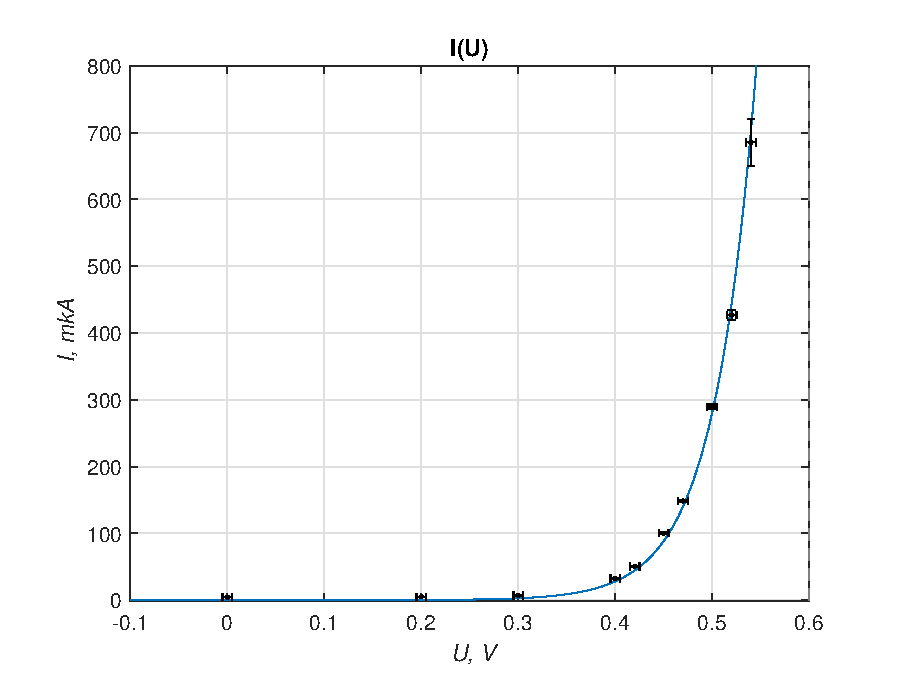
\includegraphics[scale=0.7]{vac1.eps}
\end{figure}

$\Delta I_s = \sqrt{0.139^2 + 0.035^2 + 0.005^{2}} = 0.143$нА

$\Delta m = \sqrt{0.01^{2} + 0.02^{2}} = 0.02$

$I_s = 2.833 \pm 0.143 \; \text{нА}, \; m = 1.76 \pm 0.02$


\subsection{Третій діод}

$\Delta I_s = \sqrt{3.331^2 + 0.237^2 + 0.005^{2}} = 3.339$нА

$\Delta m = \sqrt{0.04^{2} + 0.04^{2}} = 0.04$

$I_s = 14.406 \pm 3.339 \; \text{нА}, \; m = 1.99 \pm 0.06$


\newpage

% \begin{table}[ht]
% 	\centering
% 	\caption{ВАХ третього діода}
% 	\begin{tabular}{lllllll}
% 		\hline
%         $U$, В & $I_1$, мкА & $I_2$, мкА & $I_3$, мкА & $I_4$, мкА & $\sigma_{\overline{I}}$ &
%         $\Delta U$\\
% 		\hline
% 		0  & 5   & 4   & 5    & 5 & 0.2  & 0.005\\
% 		0.2  & 5   & 5   & 5    & 5 & 0  & 0.005\\
% 		0.3  & 6   & 7   & 7    & 7 & 0.2 & 0.005\\
% 		0.35 & 15  & 15  & 15   & 16 & 0.2 & 0.005\\
% 		0.4  & 45  & 46  & 46   & 48 & 0.5 & 0.005\\
% 		0.45 & 138 & 137 & 140  & 142 & 0.9 & 0.005\\
% 		0.5  & 393 & 358 & 364  & 390 & 7.7 & 0.005\\
% 		0.52 & 536 & 535 & 525  & 533 & 2.1 & 0.005\\
% 		0.54 & 840 & 870 & 886  & 900 & 11.2 & 0.005\\
% 		0.55 & 971 & 030 & 1040 & 1030 & 13.6 & 0.005\\
% 		\hline
% 	\end{tabular}
% \end{table}

\newpage
\subsection{Перший діод}
\begin{table}[!ht]
	\centering
	\caption{ВФХ першого діода}
	\begin{tabular}{lllllll}
		\hline
        $U$, В & $C_1$, мкА & $C_2$, мкА & $C_3$, мкА & $C_4$, мкА & $\sigma_{\overline{C}}$ & $\Delta U$ \\
		\hline
        -0.0  & 466 & 466 & 466 & 465 & 0.2 & 0.005\\
		-0.4  & 437 & 436 & 436 & 436 & 0.2 & 0.005\\
		-0.61 & 425 & 424 & 425 & 424 & 0.2 & 0.005\\
		-0.81 & 414 & 413 & 413 & 413 & 0.2 & 0.005\\
		-1.02 & 404 & 404 & 404 & 403 & 0.2 & 0.005\\
		-1.4  & 387 & 386 & 386 & 386 & 0.2 & 0.005\\
		-1.6  & 379 & 378 & 378 & 378 & 0.2 & 0.005\\
		-2.0  & 365 & 364 & 365 & 364 & 0.2 & 0.005\\
		-2.2  & 357 & 358 & 357 & 357 & 0.2 & 0.005\\
		-2.5  & 349 & 349 & 349 & 352 & 0.6 & 0.005\\
		-3.0  & 335 & 335 & 335 & 334 & 0.2 & 0.005\\
		-4.0  & 312 & 312 & 312 & 312 & 0 & 0.005\\
		\hline
	\end{tabular}
\end{table}
\begin{figure}[!ht]
    \centering
    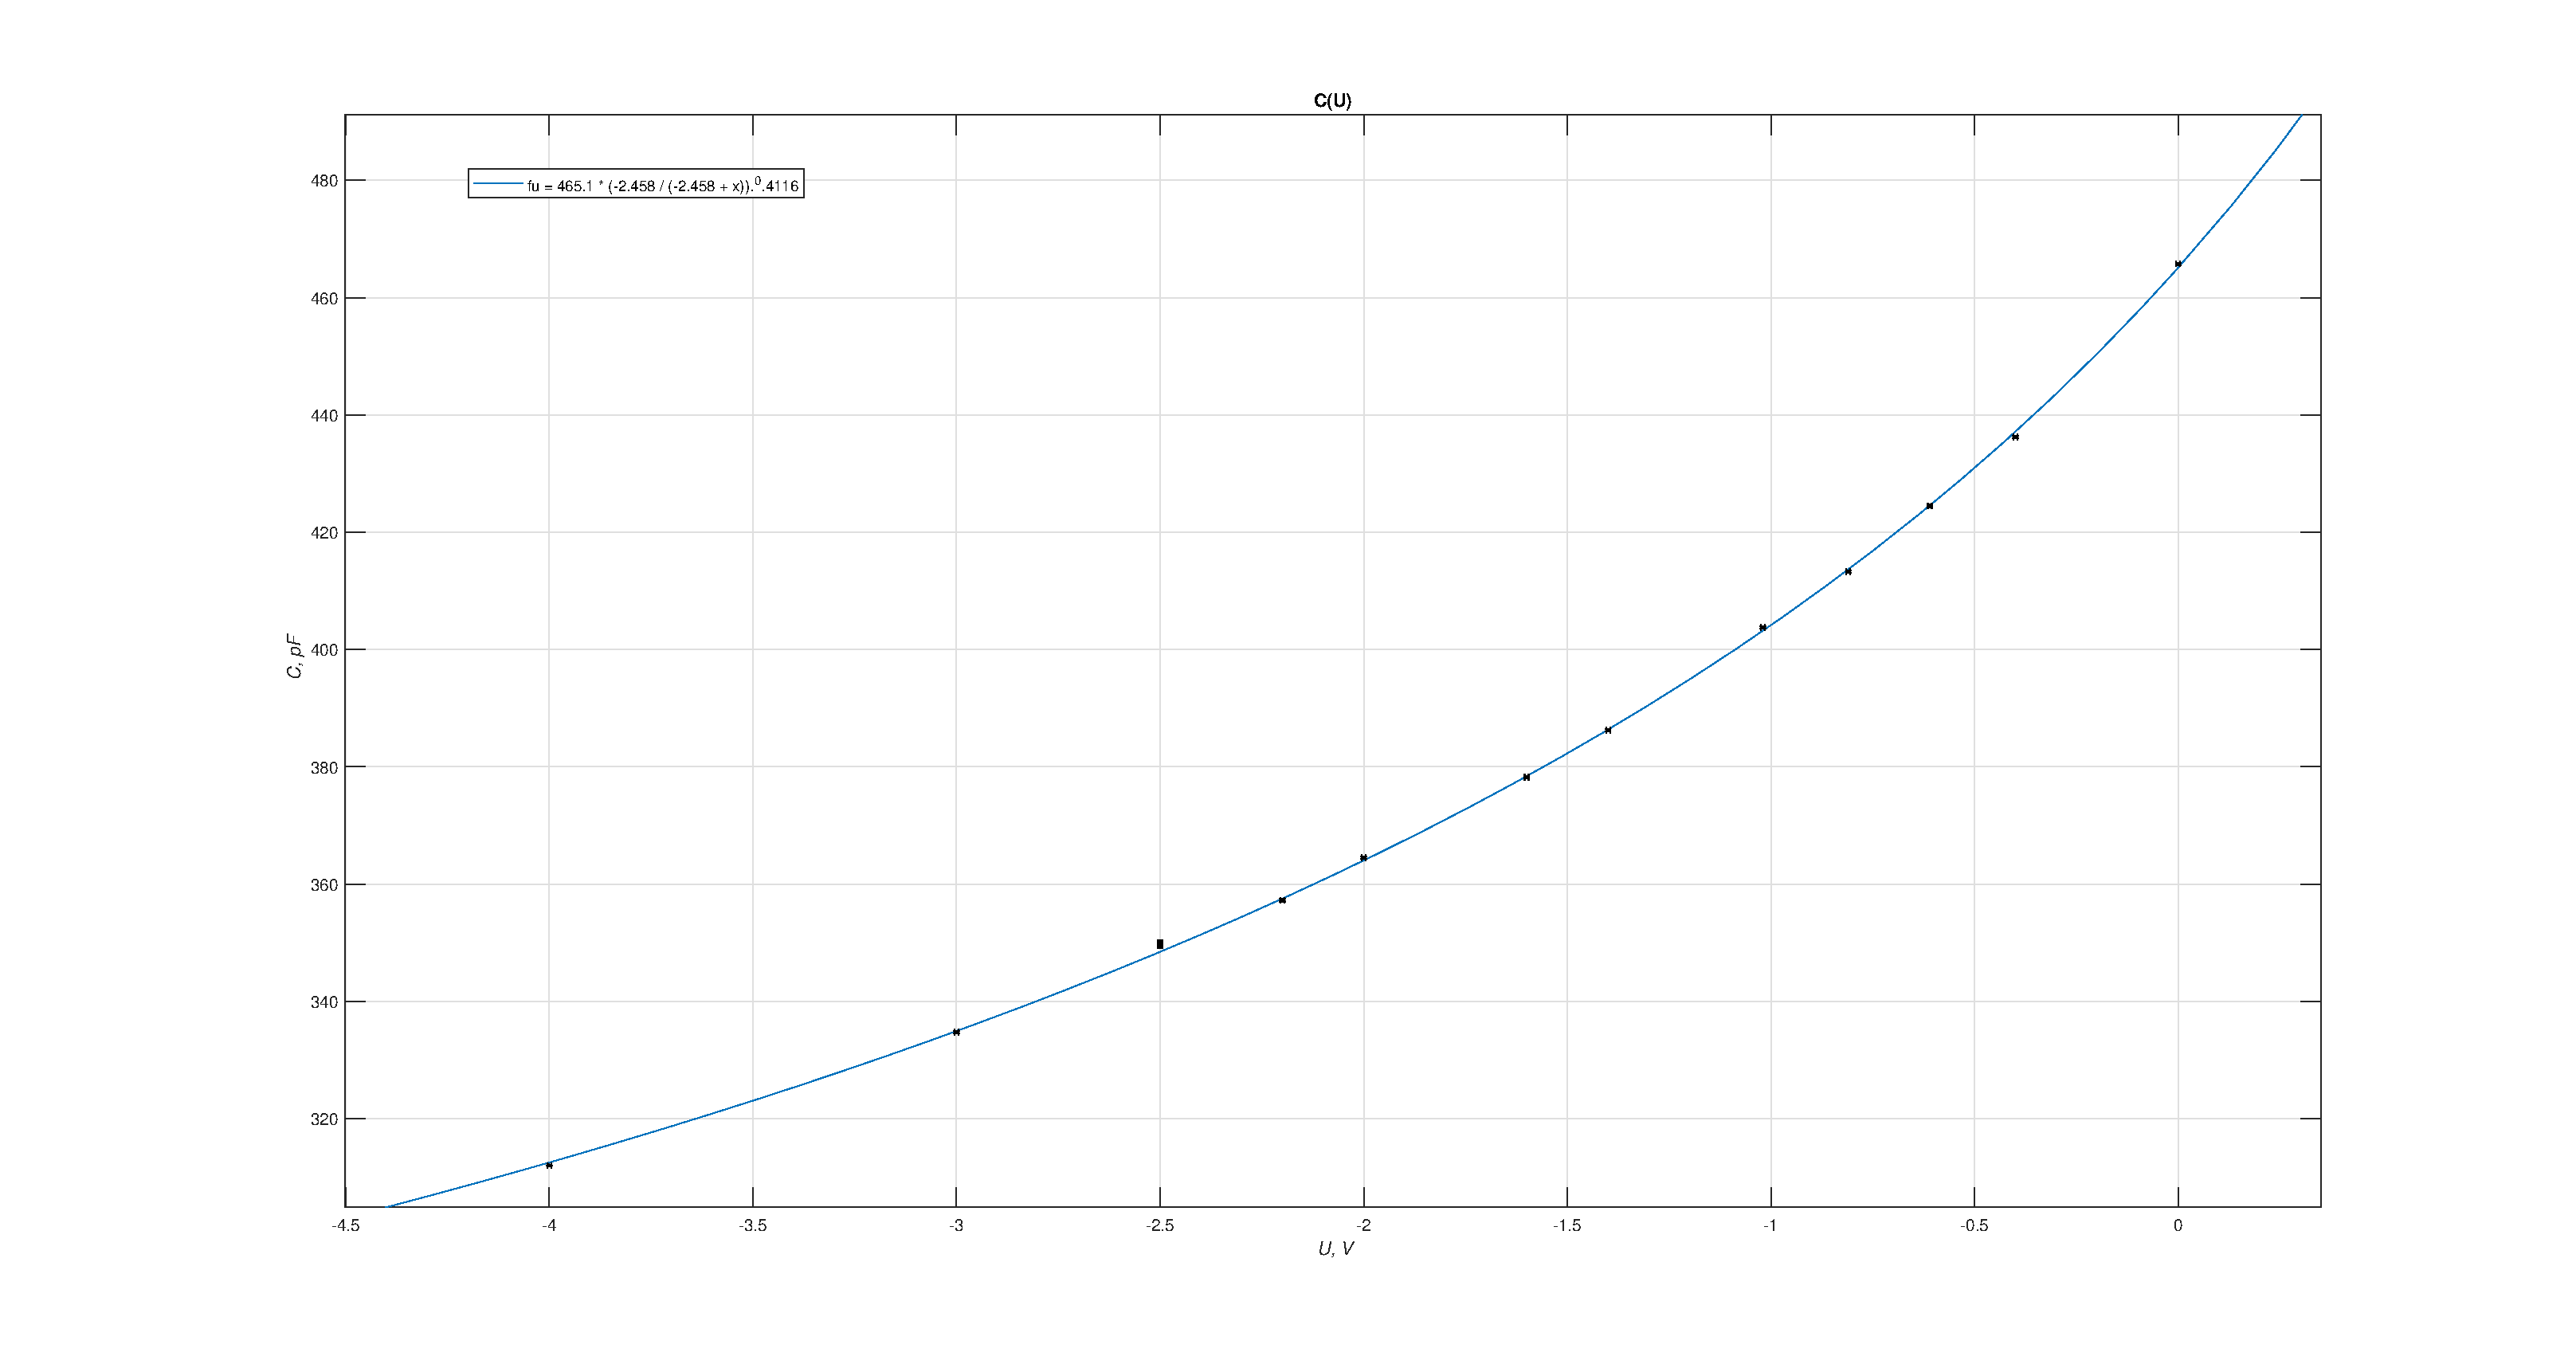
\includegraphics[scale=0.25]{vfc_0.eps}
\end{figure}


$\Delta \varphi_k = \sqrt{0.03^{2} + 0.02^{2}} = 0.04$

$\Delta \nu = \sqrt{0.004^{2} + 0.003^{2}} = 0.005$

$\varphi_k = 2.46 \pm 0.04 \; \text{В}, \; \nu = 0.412 \pm 0.0005$


\subsection{Другий діод}
\begin{align*}
C(U) = C_0 = const\\
C_0 = 11 \; \text{мкФ}.
\end{align*}


\newpage
\subsection{Третій діод}
Установка дозволила визначити лише декілька точок, тому дані не достовірні

\begin{table}[h!]
	\centering
	\caption{ВФХ третього діода}
	\begin{tabular}{lllllll}
		\hline
        $U$, В & $C_1$, мкА & $C_2$, мкА & $C_3$, мкА & $C_4$, мкА & $\sigma_{\overline{C}}$  & $\Delta U$\\
		\hline
%		1.97 $\pm$ 0.005 & 46 & 52 & 53 & 53 &  \\
%		1.95 $\pm$ 0.005 & 35 & 38 & 35 & 38 &  \\
%		1.88 $\pm$ 0.005 & 22 & 23 & 23 & 23 &  \\
%		1.72 $\pm$ 0.005 & 20 & 20 & 20 & 20 &  \\
%		0.9 $\pm$ 0.005 & 17 & 17 & 17 & 17 &  \\
		0.00  & 15 & 15 & 15 & 15 & 0 & 0.005\\
		-0.5  & 15 & 15 & 15 & 15 & 0 & 0.005\\
		-2.25  & 14 & 14 & 14 & 14 & 0 & 0.005\\
		-6.3  & 13 & 13 & 13 & 13 & 0 & 0.005\\
		-10  & 12 & 12 & 12 & 12 & 0 & 0.005\\
		\hline
	\end{tabular}
\end{table}
\begin{figure}[!ht]
    \centering
    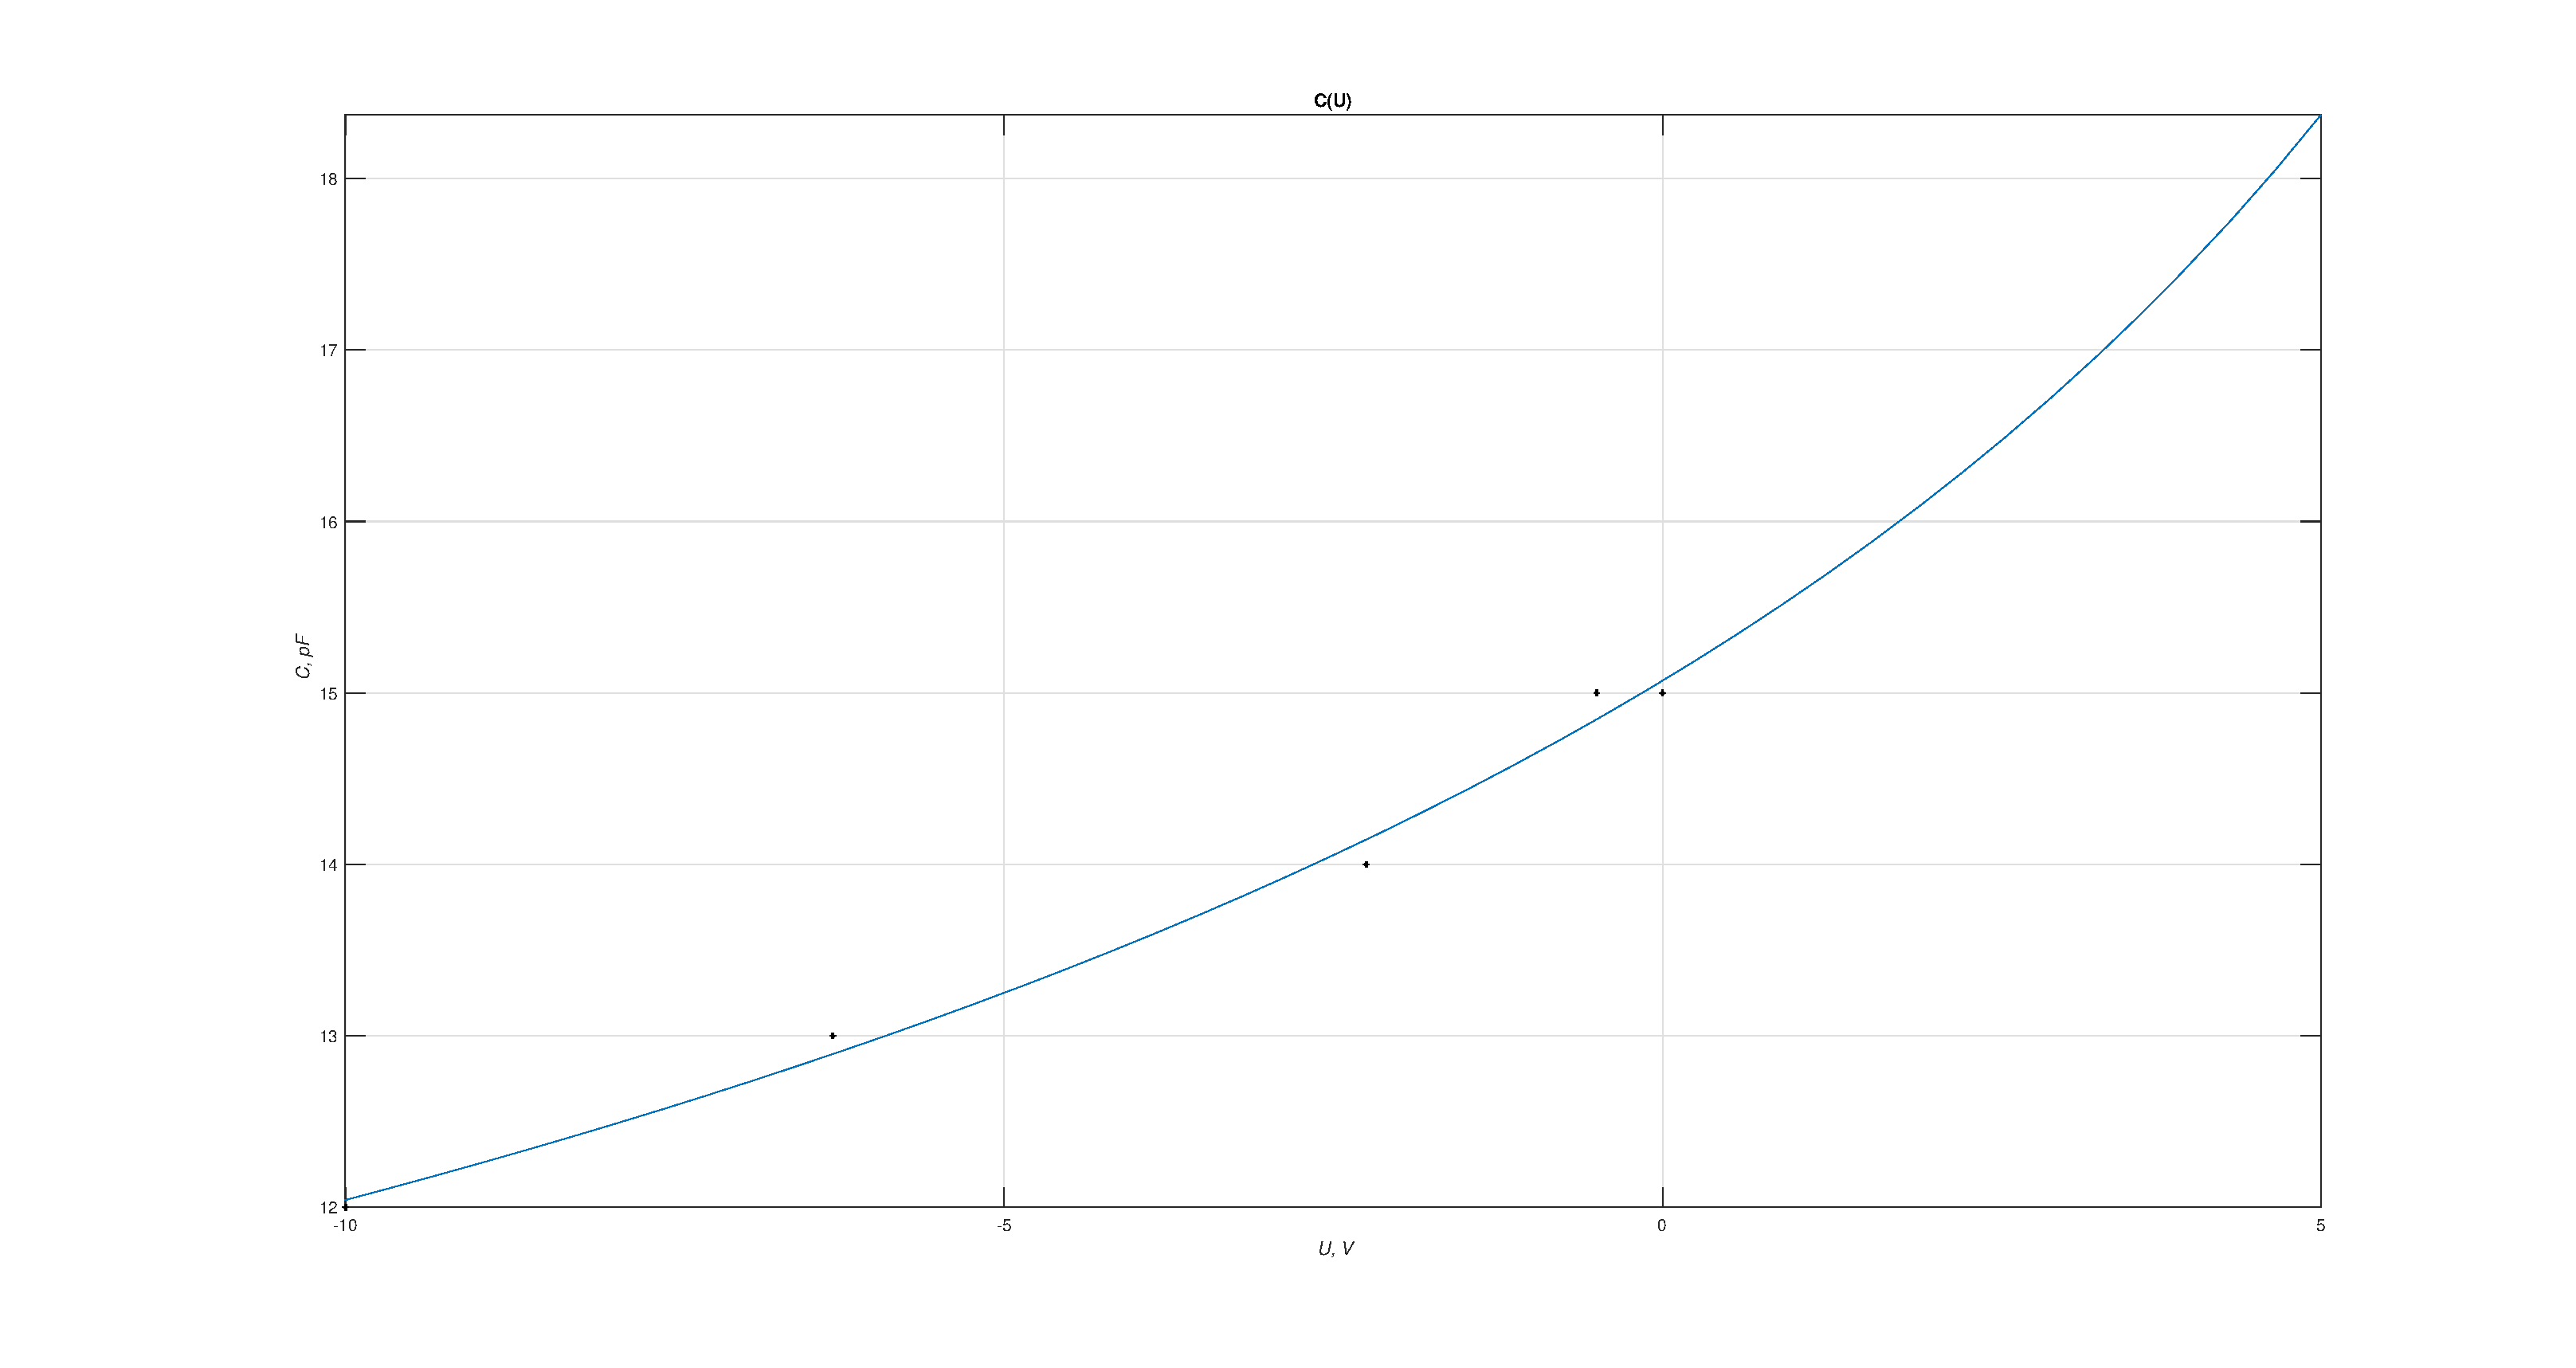
\includegraphics[scale=0.25]{vfc_2.eps}
\end{figure}


$\varphi_k = -12.144 \; \text{В}, \; \nu = 0.3733$.

\section{Визначення диференціального опору діода}
Диференціальний опір діоду визначається за формулою:
\[
    R = \dfrac{d U}{d I}.
\]
Або маючи експериментальні точки замінимо $dU$ на $\Delta U$ на $dI$ на $\Delta I$:
\[
	R = \dfrac{\Delta U}{\Delta I}.
\]

Задля забезпечення найбільш можливої точності, візьмемо точки, що розташовані на найбільш гладкій ділянці кривої.

Отже, можемо значення:

\begin{itemize}
    \item $R_1 = 85714,2857 \; \text{Ом}$
    \item $R_2 = 36363,6364 \; \text{Ом}$
    \item $R_3 = 57142,8571 \; \text{Ом}$
\end{itemize}

\newpage
\section{Висновок}

З результатів експерименту маємо

\begin{enumerate}
    \item
        Германієвий
    \item
        Кремнієвий
    \item
        Германієвий
\end{enumerate}

Експеримент підтвердив теоретичні закони для вольт парадних та вольт оперних характеристик діодів.
З апроксимації цих залежностей визначається тип діода, диференціальний опір та контактна різниця
потенціалів.

На точність результатів вплинув доволі вузький спектр напруг.


\section{Контрольні запитання:}
\begin{enumerate}
    \item {
        \bfНапівпровідники n та p типу. Напівкласична теорія p-n переходу.}\\
    Напівпровідник n-типу -- це напівпровідник, основними носіями заряду в якому є електрони.\\
    Напівпровідник p-типу -- це напівпровідник, основними носіями заряду в якому являються дірки.\\
    P-n перехід -- область контакту напівпровідників p- та n-типу, в якій відбувається перехід від одного типу провідності до іншого. Ця область характеризується одностороннім пропусканням електричного струму.
    \item
        {\bfЯк виникає р-n перехід при ідеальному контакті напівпровідників з
різним типом електропровідності.}\\
    Якщо створити ідеальний контак між напівпровідниками, то утвориться дифузійний струм, в результаті якого дірки та електрони почнуть перетікати туди де їх концентрація менше допоки не встановиться рівновага. Таким чином на межі контакту, в провіднику p-типу виникає шар електронів (негативний заряд), а в провіднику n-типу виникає шар дірок(позитивний заряд).
    \item
        {\bfНамалювати схему і пояснити спосіб зняття ВАХ діодів за допомогою
амперметра і вольтметра.}
    \begin{figure}[!ht]
      \centering
      \includegraphics[scale=0.6]{VAC.jpg}
    \end{figure}
    \item
        {\bfПояснити роботу р-n переходу при прямому і зворотному включенні.}\\
    Пряме включення напівпровідника означає підключення позитивного полюса джерела живлення до p-облатсі напівпровідника, а негативного полюса - до n-області напівпровідника. Пряме включення створює зовнішнє електричне поле, що напрямлено назустріч електричному полю діода. Це спричиняє збільшення дифузійного струму. Також приводить до зменшення замикаючого шару.\\
    Зворотнє включення напівпровідника означає підключення позитивного полюса джерела живлення до n-облатсі напівпровідника, а негативного полюса - до p-області напівпровідника. Зовнішнє електричне поле напрямлене в той самий бік що і власне. Це призводить до зростання потенціального бар'єру та зменшення ширини замикаючого шару.
    \item
        {\bfЧим відрізняються ВАХ ідеального р-n переходу і реального діода.}\\
    Для ідеального діода опір при $U < 0$ набуває значення $R = \infty $, тому лінія сили струму співпадає з віссю абсцис, а при $U \geq 0 $ -- $ R = 0. \Rightarrow I=\infty$
    \item
        {\bfДати визначення диференціального опору діода і пояснити графічно
спосіб його визначення.}\\
    Диференціальний опір діода $R=\dfrac{dU}{dI}$. Застосовується тому, що для нелінійних елементів ВАХ не описується законом ома, тому звичайний опір виористовувати не можна.\\
    Графічне знаходження диференціального опору заключажться в знаходженні тангенса кута нахилу прямої між двума сусідніми точками на графіку ВАХ.
    \item
        {\bfНамалювати ВАХ стабілітрона і визначити робочу ділянку ВАХ при
стабілізації напруги.}\\
    \begin{figure}[!ht]
      \centering
      \includegraphics[scale=0.8]{problem8.jpg}
    \end{figure}
    \item
        {\bfЧому величина бар'єрної ємності залежить від прикладеної напруги?}\\
    Бар'єрна ємність це ємність конденсатора, що складається з напівпровдників. А оскільки ємність конденсатора залежить від напруги, то бар'єрна ємність залежить також.
    \item
        {\bfЯка фізична природа дифузійної ємності р-n переходу?}\\
    Дифузійна ємність виникає за рахунок накопичення негативних зарядів в p-області та позитивних в n-області.
    \item
        {\bfПерерахувати основні параметри діодів.}\\
    Струм насичення, контактний потенціал, ємність при нульовій зворотній напрузі.
\end{enumerate}

\end{document}



